\documentclass{article}

% if you need to pass options to natbib, use, e.g.:
%     \PassOptionsToPackage{numbers, compress}{natbib}
% before loading neurips_2019

% ready for submission
% \usepackage{neurips_2019}

% to compile a preprint version, e.g., for submission to arXiv, add add the
% [preprint] option:
     \usepackage[preprint]{neurips_2019}

% to compile a camera-ready version, add the [final] option, e.g.:
%     \usepackage[final]{neurips_2019}

% to avoid loading the natbib package, add option nonatbib:
%     \usepackage[nonatbib]{neurips_2019}

\usepackage[utf8]{inputenc} % allow utf-8 input
\usepackage[T1]{fontenc}    % use 8-bit T1 fonts
\usepackage{hyperref}       % hyperlinks
\usepackage{url}            % simple URL typesetting
\usepackage{booktabs}       % professional-quality tables
\usepackage{amsfonts}       % blackboard math symbols
\usepackage{nicefrac}       % compact symbols for 1/2, etc.
\usepackage{microtype}      % microtypography

% Not part of the offical NeurIPS template
\usepackage{censor}
\usepackage{amssymb}
\usepackage{amsthm}
\usepackage{mathtools}
\usepackage{xfrac}
\usepackage{caption}
\usepackage{subcaption}
\usepackage{float}
\usepackage{caption}

\title{Neural Arithmetic Units}

% The \author macro works with any number of authors. There are two commands
% used to separate the names and addresses of multiple authors: \And and \AND.
%
% Using \And between authors leaves it to LaTeX to determine where to break the
% lines. Using \AND forces a line break at that point. So, if LaTeX puts 3 of 4
% authors names on the first line, and the last on the second line, try using
% \AND instead of \And before the third author name.

\author{%
  Andreas Madsen$^{\dag\ddag}$ \\
  \texttt{amwebdk@gmail.com}
  \AND
  Alexander Rosenberg Johansen$^{\dag}$ \\
  \texttt{alexander@herhjemme.dk} \\
  \AND
  Who else? \\
  \\
$^\dag$Technical University of Denmark \quad
$^\ddag$Computationally Demanding
}

\begin{document}
\StopCensoring % NOTE, remove for peer-review to ensure anonymity.

\maketitle

\begin{abstract}
Neural networks often perform extremely when interpolating within the numerical range of the training dataset. However, when extrapolating outside this range they often fail, because the neural network have learned an approximation and not the exact rule. Previous work on neural arithmetic logic unit (NALU), attempts to solve this issue by learning exact arithmetic operations. Those results are unfortunately extremely difficult to reproduce consistently. In this paper we propose two alternative arithmetic units, one for addition and one for multiplication. We show that these units have fewer parameters, converges much more consistently, learns faster that previous arithmetic units, and the weight have meaningful discrete values.
\end{abstract}

\section{Introduction}
When studying intelligence, insects, reptiles, and humans have been found to possess neurons with the capacity to hold integers, real numbers, and perform arithmetic operations \cite{nieder-neuronal-number,rugani-arithmetic-chicks,gallistel-numbers-in-brain}.
In our quest to mimic intelligence we have put much faith in neural networks, which in turn has provided unparalleled and often superhuman performance in tasks requiring high cognitive abilities \cite{natureGo,bert,openai-learning-dexterous}.
However, when using neural networks to learn simple arithmetic problems, such as counting, multiplication, or comparison they systematically fail to extrapolate onto unseen ranges \cite{stillNotSystematic,suzgun2019evaluating,trask-nalu}.
The absence of inductive bias makes it difficult for neural networks to extrapolate well on arithmetic tasks as they lack the underlying logic to represent the required operations.

We would like to achieve a neural network component that can take an arbitrary hidden input, learn to select the appropriate elements, and apply the desired arithmetic operation.
A recent attempt to achieve this goal is the Neural Arithmetic Logic Unit (NALU), by \citet{trask-nalu}.

The NALU consists of two sub-units: the $\text{NAC}_{+}$ for addition/subtraction and the $\text{NAC}_{\bullet}$ for multiplication/division.
The sub-units are softly gated using a sigmoid function in order to exclusively select one of the sub-units.
However, we find that the soft gating mechanism and the $\text{NAC}_{\bullet}$ are fragile and hard learn.

In this paper, we analyze and improve upon the $\text{NAC}_{+}$ and $\text{NAC}_{\bullet}$ with respect to addition, subtraction, and multiplication.
Our proposed improvements, namely the Neural Addition Unit (NAU) and Neural Multiplication Unit (NMU), are more theoretically founded and improves performance regarding stability, speed of convergence, and interpretability of results.
Most importantly, the NMU can support a large hidden input-size.

The improvements, based on a theoretical analysis of the NALU and its components, are achieved by a simplification of the parameter matrix for a better gradient signal, a sparsity regularizer, and a new multiplication unit that can be optimally initialized and supports both negative and small numbers.
The NMU does not support division.
However, we find that the $\text{NAC}_{\bullet}$ in practice also only supports multiplication and cannot learn division (for theoretical findings on why division is hard to learn, see section \ref{sssec:nac-mul}).

To analyze the impact of each improvement in the NMU by introducing several variants of the $\text{NAC}_{\bullet}$.
We find that, allowing division makes optimization for multiplication harder, linear and regularized weights improve convergence, and that the NMU style of multiplication is critical when increasing the hidden size.

Furthermore, we improve upon existing benchmarks in \citet{trask-nalu} by expanding the ``simple function task'', using a multiplicative variant of ``MNIST Counting and Arithmetic Tasks'', and use an improved success-criterion \citet{maep-madsen-johansen-2019}.
A success-criterion is important because the arithmetic layers are solving a logical problem.
We propose the MNIST multiplication variant as we want to test the NMU's and $\text{NAC}_{\bullet}$'s ability to learn from real data.
%Hence, the solution found is either correct or wrong.
%To test this we propose using a success-criteria to evaluate model performance.
%A success-criterion enables measuring sensitivity to the initialization seed as well as the number of iterations until convergence.

\begin{figure}[t]
\centering
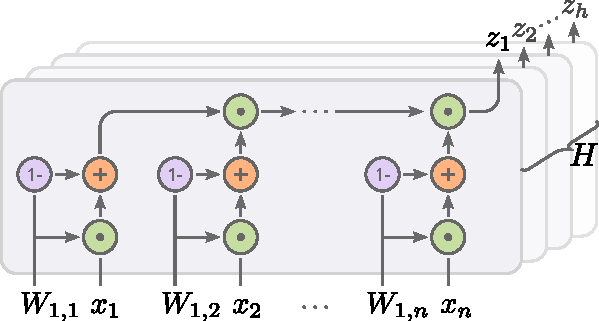
\includegraphics[scale=0.7]{graphics/nmu.pdf}
\caption{Visualization of NMU for a single output scalar $z_1$, this construction repeats for every element in the output vector $\mathbf{z}$.}
\end{figure}

\subsection{Learning a 10 parameter function}
Consider the static function $t = (x_1 + x_2) \cdot (x_1 + x_2 + x_3 + x_4)$ for $x \in \mathbb{R}^4$. To illustrate the ability of $\mathrm{NAC}_{\bullet}$, NALU, and our proposed NMU, we conduct 100 experiemnts for each model, where we attempt to fit this function. Table \ref{tab:very-simple-function-results} show that NMU has a higher success rate and converges faster.
%When inspecting the $6\%$ that did not converge, we found the issue to be underflow when $w = 0$ in the multiplication layer.
\begin{table}[!h]

\caption{\label{tab:very-simple-function-results}Shows the success-rate, at what global step the model converged at, and the sparsity error for all weight matrices, with 95\% confidence interval. Best result is highlighed.}
\centering
\begin{tabular}{crllll}
\toprule
\multicolumn{1}{c}{Op} & \multicolumn{1}{c}{Model} & \multicolumn{1}{c}{Success} & \multicolumn{2}{c}{Solved at} & \multicolumn{1}{c}{Sparsity error} \\
\cmidrule(l{3pt}r{3pt}){1-1} \cmidrule(l{3pt}r{3pt}){2-2} \cmidrule(l{3pt}r{3pt}){3-3} \cmidrule(l{3pt}r{3pt}){4-5} \cmidrule(l{3pt}r{3pt}){6-6}
 &  & Rate & Median & Mean & Mean\\
\midrule
 & $\mathrm{NAC}_{\bullet}$ & $13\% {~}^{+8\%}_{-5\%}$ & $5.5 \cdot 10^{4}$ & $5.9 \cdot 10^{4} {~}^{+7.8 \cdot 10^{3}}_{-6.6 \cdot 10^{3}}$ & $7.5 \cdot 10^{-6} {~}^{+2.0 \cdot 10^{-6}}_{-2.0 \cdot 10^{-6}}$\\

 & NALU & $26\% {~}^{+9\%}_{-8\%}$ & $7.0 \cdot 10^{4}$ & $7.8 \cdot 10^{4} {~}^{+6.2 \cdot 10^{3}}_{-8.6 \cdot 10^{3}}$ & $9.2 \cdot 10^{-6} {~}^{+1.7 \cdot 10^{-6}}_{-1.7 \cdot 10^{-6}}$\\

\multirow{-3}{*}{\centering\arraybackslash $\bm{\times}$} & NMU & $\mathbf{94\%} {~}^{+3\%}_{-6\%}$ & $\mathbf{1.4 \cdot 10^{4}}$ & $\mathbf{1.4 \cdot 10^{4}} {~}^{+2.2 \cdot 10^{2}}_{-2.1 \cdot 10^{2}}$ & $\mathbf{2.6 \cdot 10^{-8}} {~}^{+6.4 \cdot 10^{-9}}_{-6.4 \cdot 10^{-9}}$\\
\bottomrule
\end{tabular}
\end{table}


\section{Improving NAC and NALU}

The NALU from \cite{trask-nalu} is a neural unit capable of doing either exact addition or multiplication, controlled by a sigmoid-gating-mechanism. The addition part is trivial, as this is just a matrix multiplication $\mathbf{a} = \mathbf{W}\mathbf{x}$. The only special part is that the weight matrix $\mathbf{W}$ is constrained to be between $-1$ and $1$. This this done using a $\mathbf{W} = \mathrm{tahn}({\hat{\mathbf{W}}}) \sigma({\hat{\mathbf{M}}})$ construction. Meaning that the weight matrix $\mathbf{W}$ is not trained directly, but computed from two auxiliary weight matrices. The core idea is that $\hat{\mathbf{W}}$ controls the sign and $\hat{\mathbf{M}}$ controls if the weight is zero. One of their core claims, is that this weight matrix construction have a sparse bias, which improves extrapolation for cases where a sparse weight is part of the underlying model.

For the multiplication, an exponential-log transformation is used in order to do exact multiplication (within $\epsilon$ precision) using a matrix multiplication, $\mathbf{m} = \exp(\mathbf{W} \log(|\mathbf{x}| + \epsilon))$.

The addition unit (originally named NAC), and the multiplication unit are in themselves theoretically applicable in any neural network as well as being differentiable. The NALU, then combines them using a sigmoid-gating-mechanism\footnote{The lack of bias term is not a typo. Our preliminary investigations suggests that this is a hack to increase extrapolation of the gate. However in this paper the focus is only arithmetic operators themself.} $\mathbf{g} = \sigma(\mathbf{G} \mathbf{x})$ that chooses softly between addition and multiplication $\mathbf{z} = \mathbf{g} \odot \mathbf{a} + (1 - \mathbf{g}) \odot \mathbf{m}$.

In terms of the theory, the Original NALU paper \cite{trask-nalu} does not discuss anything more than mentioned so-far in this paper. To aid discussion of why this particular construction problematic, and also suggests improvements which will be empirically validated later, the NAC and its multiplication variant is re-formulated using scalar notation.

\begin{equation}
\begin{aligned}
&W_{h_\ell, h_{\ell-1}} = \tanh(\hat{W}_{h_\ell, h_{\ell-1}}) \sigma(\hat{M}_{h_\ell, h_{\ell-1}}) \\
\textrm{NAC}_+:\ &z_{h_\ell} = \sum_{h_{\ell-1}=1}^{H_{\ell-1}} W_{h_{\ell}, h_{\ell-1}} z_{h_{\ell-1}} \\
\textrm{NAC}_\bullet:\ &z_{h_\ell} = \exp\left(\sum_{h_{\ell-1}=1}^{H_{\ell-1}} W_{h_{\ell}, h_{\ell-1}} \log(|z_{h_{\ell-1}}| + \epsilon) \right)
\end{aligned}
\end{equation}

\subsection{Weight matrix construction}

The weight matrix constructions $\mathrm{tahn}({\hat{\mathbf{W}}}) \sigma({\hat{\mathbf{M}}})$ have a few issues worth mentioning. First, the loss gradient with respect to the weight matrices, can without loss of generality, easily be derived to:

\begin{equation}
\begin{aligned}
\frac{\partial \mathcal{L}}{\partial \hat{W}_{h_{\ell-1},h_\ell}} &= \frac{\partial \mathcal{L}}{\partial W_{h_{\ell-1},h_\ell}} (1 - \tanh^2(\hat{W}_{h_{\ell-1},h_\ell})) \sigma(\hat{M}_{h_{\ell-1},h_\ell}) \\
\frac{\partial \mathcal{L}}{\partial \hat{M}_{h_{\ell-1},h_\ell}} &= \frac{\partial \mathcal{L}}{\partial W_{h_{\ell-1},h_\ell}} \tanh(\hat{W}_{h_{\ell-1},h_\ell}) \sigma(\hat{M}_{h_{\ell-1},h_\ell}) (1 - \sigma(\hat{M}_{h_{\ell-1},h_\ell}))
\end{aligned}
\end{equation}

This reveals that this construction is particularly problematic, as $E[\mathrm{tahn}(\hat{W}_{h_{\ell-1},h_\ell})] = 0$ when $E[\hat{W}_{h_{\ell-1},h_\ell}] = 0$. Initializing $\hat{W}_{h_{\ell-1},h_\ell}$ to have zero expectation, is not just common choice but necessary in order to achieve $E[W_{h_{\ell-1},h_\ell}] = 0$, which is necessary to get desired property $E[z_{h_\ell}] = 0$ in linear units such as as the NAC \cite{glorot-initialization}.

The NALU \cite{trask-nalu} paper also claims that this weight matrix construction, creates a bias for $\{-1, 0, 1\}$. However, they provide no empirically or theoretical evidence to support that. In our own empirical investigation as seen in the experiments section, we also find no support for that claim.

To improve on both of these failings, we propose a simple clamped linear construction instead, that is regularize to have the desired bias of $\{-1, 0, 1\}$ and have gradient outside of $[-1, 1]$.

\begin{equation}
\begin{aligned}
&W_{h_{\ell-1},h_\ell} = \min(\max(\hat{W}_{h_{\ell-1},h_\ell}, -1), 1), \\
&\mathcal{R}_{\ell,\mathrm{bias}} = \frac{1}{H_\ell + H_{\ell-1}} \sum_{h_\ell=1}^{H_\ell} \sum_{h_{\ell-1}=1}^{H_{\ell-1}} \hat{W}_{h_{\ell-1},h_\ell}^2 (1 - |\hat{W}_{h_{\ell-1},h_\ell}|)^2 \\
&\mathcal{R}_{\ell,\mathrm{oob}} = \frac{1}{H_\ell + H_{\ell-1}} \sum_{h_\ell=1}^{H_\ell} \sum_{h_{\ell-1}=1}^{H_{\ell-1}} \max(|\hat{W}_{h_{\ell-1},h_\ell}| - 1, 0)^2 \\
\textrm{NAU}:\ &z_{h_\ell} = \sum_{h_{\ell-1}=1}^{H_{\ell-1}} W_{h_{\ell}, h_{\ell-1}} z_{h_{\ell-1}} \\\end{aligned}
\end{equation}

Note that while the bias regularizer $\mathcal{R}_{\ell,\mathrm{bias}}$ also regularize $\hat{W}_{h_{\ell-1},h_\ell}$ to not be outside of $[-1, 1]$, one may choose a small regularization constant for this, or scale it up gradually as done in the experiments later. However, $\mathcal{R}_{\ell,\mathrm{oob}}$ should always be present as it is never desired to have $\hat{W}_{h_{\ell-1},h_\ell} \not\in [-1, 1]$.

\subsection{Multiplication unit}

The multiplication unit has its own issues. It should be easy to see that when $|z_{h_{\ell-1}}|$ is near zero and when $\hat{W}_{h_{\ell-1},h_\ell}$ is near $-1$ the $z_{h_\ell}$ value explodes. However, the issue extends beyond a weight near $-1$ as is revealed in the gradients, especially the backpropergation term $\frac{\partial z_{h_\ell}}{\partial z_{h_{\ell-1}}}$:

\begin{equation}
\begin{aligned}
\frac{\partial \mathcal{L}}{\partial W_{h_{\ell}, h_{\ell - 1}}} &= \frac{\partial \mathcal{L}}{\partial z_{h_\ell}} \frac{\partial z_{h_\ell}}{\partial W_{h_{\ell}, h_{\ell - 1}}} = \frac{\partial \mathcal{L}}{\partial z_{h_\ell}} z_{h_\ell} \log(|z_{h_{\ell-1}}| + \epsilon) \\
\frac{\partial \mathcal{L}}{\partial z_{h_{\ell-1}}} &= \sum_{h_\ell = 1}^{H_\ell} \frac{\partial \mathcal{L}}{\partial z_{h_\ell}} \frac{\partial z_{h_\ell}}{\partial z_{h_{\ell-1}}} = \sum_{h_\ell = 1}^{H_\ell} \frac{\partial \mathcal{L}}{\partial z_{h_\ell}} z_{h_\ell} W_{h_\ell, h_{\ell-1}} \frac{\mathrm{sign}(z_{h_{\ell-1}})}{|z_{h_{\ell-1}}| + \epsilon}
\end{aligned}
\end{equation}

In should be clear from $\frac{\mathrm{sign}(z_{h_{\ell-1}})}{|z_{h_{\ell-1}}| + \epsilon}$ that for $z_{h_{\ell-1}}$ near zero, the backpropagation term will not only explode, but can oscillate between a large postive value and large negative value, which is very problematic in optimization \cite{adam-optimization}. This issue does not only exists for $|z_{h_{\ell-1}}| < \epsilon$, which may have a small probability if $z_{h_{\ell-1}}$ has a wide distribution. But is can also be an issue for values outside of this interval as seen in figure \ref{fig:nac-mul-eps-issue}.

\begin{figure}[H]
\centering
\begin{subfigure}{.33\textwidth}
  \centering
  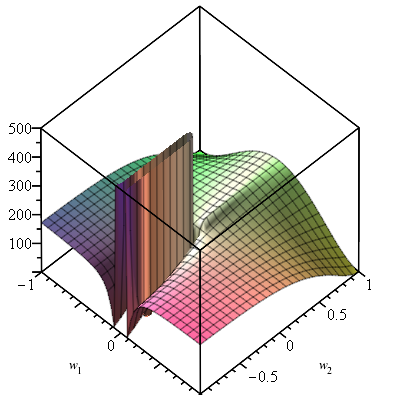
\includegraphics[width=\linewidth]{graphics/nac-mul-eps-1em7.png}
  \caption{$\epsilon = 10^{-7}$}
\end{subfigure}%
\begin{subfigure}{.33\textwidth}
  \centering
  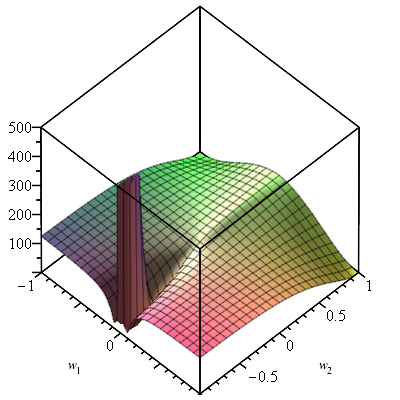
\includegraphics[width=\linewidth]{graphics/nac-mul-eps-1em1.png}
  \caption{$\epsilon = 0.1$}
\end{subfigure}
\begin{subfigure}{.33\textwidth}
  \centering
  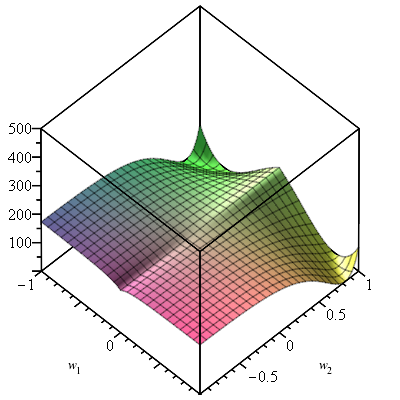
\includegraphics[width=\linewidth]{graphics/nac-mul-eps-1.png}
  \caption{$\epsilon = 1$}
\end{subfigure}
\caption{RMS loss curvature for a $\mathrm{NAC}_{+}$ layer followed by a $\mathrm{NAC}_{\bullet}$ layer. The weight matrices constrained are to $\mathbf{W}_1 = \left[\protect\begin{smallmatrix}
w_1 & w_1 & 0 & 0 \\
w_1 & w_1 & w_1 & w_1
\protect\end{smallmatrix}\right]$, $\mathbf{W}_2 = \left[\protect\begin{smallmatrix}
w_2 & w_2
\protect\end{smallmatrix}\right]$. The problem is $x = \left(1, 1.2, 1.8, 2\right), t = 11.25$. Desired solution is $w_1 = w_2 = 1$, although this problem have additional undesired solutions.}
\label{fig:nac-mul-eps-issue}
\end{figure}

These observations are particular problematic when considering that $E[z_{h_{\ell-1}}] = 0$ is a desired property when initializing \cite{glorot-initialization}. An alternative multiplication operator must thus be able to not explode for $z_{h_{\ell-1}}$ near zero. To that end we propose a new neural multplication units (NMU): 

\begin{equation}
\begin{aligned}
&W_{h_{\ell-1},h_\ell} = \min(\max(\hat{W}_{h_{\ell-1},h_\ell}, 0), 1), \\
&\mathcal{R}_{\ell,\mathrm{bias}} = \frac{1}{H_\ell + H_{\ell-1}} \sum_{h_\ell=1}^{H_\ell} \sum_{h_{\ell-1}=1}^{H_{\ell-1}} \hat{W}_{h_{\ell-1},h_\ell}^2 (1 - \hat{W}_{h_{\ell-1},h_\ell})^2 \\
&\mathcal{R}_{\ell,\mathrm{oob}} = \frac{1}{H_\ell + H_{\ell-1}} \sum_{h_\ell=1}^{H_\ell} \sum_{h_{\ell-1}=1}^{H_{\ell-1}} \max\left(\left|\hat{W}_{h_{\ell-1},h_\ell} - \frac{1}{2}\right| - \frac{1}{2}, 0\right)^2 \\
\textrm{NMU}:\ &z_{h_\ell} = \prod_{h_{\ell-1}=1}^{H_{\ell-1}} \left(W_{h_{\ell-1},h_\ell} z_{h_{\ell-1}} + 1 - W_{h_{\ell-1},h_\ell} \right)
\end{aligned}
\end{equation}

This units does not support division. But supporting division is likely infeasible if $z_{h_{\ell-1}}$ near zero should not cause explosions. The NALU paper also shows that division doesn't work well for their unit, hence very little is lost here \cite{trask-nalu}. On the other hand, this unit construction understand the difference between a negative and a positive $z_{h_{\ell-1}}$ values, which should be considered an added bonus,as this allows extrapolations into the negative input range.

The gradients weight gradient and backpropagation term of the NMU are:
\begin{equation}
\begin{aligned}
\frac{\partial \mathcal{L}}{\partial W_{h_{\ell}, h_{\ell - 1}}} &= \frac{\partial \mathcal{L}}{\partial z_{h_\ell}} \frac{\partial z_{h_\ell}}{\partial W_{h_{\ell}, h_{\ell - 1}}} = \frac{\partial \mathcal{L}}{\partial z_{h_\ell}} \frac{z_{h_\ell}}{W_{h_{\ell-1},h_\ell} z_{h_{\ell-1}} + 1 - W_{h_{\ell-1},h_\ell}} \left(z_{h_{\ell-1}} - 1\right) \\
\frac{\partial \mathcal{L}}{\partial z_{h_{\ell-1}}} &= \sum_{h_\ell = 1}^{H_\ell} \frac{\partial \mathcal{L}}{\partial z_{h_\ell}} \frac{\partial z_{h_\ell}}{\partial z_{h_{\ell-1}}} = \sum_{h_\ell = 1}^{H_\ell} \frac{z_{h_\ell}}{W_{h_{\ell-1},h_\ell} z_{h_{\ell-1}} + 1 - W_{h_{\ell-1},h_\ell}} W_{h_{\ell-1},h_\ell}
\end{aligned}
\end{equation}

These is much more well-behaved. Note also that the fraction does not explode for $z_{h_{\ell-1}}$ close to zero, as the denominator simply cancels out a term in $z_{h_\ell}$.

\begin{figure}[H]
\centering
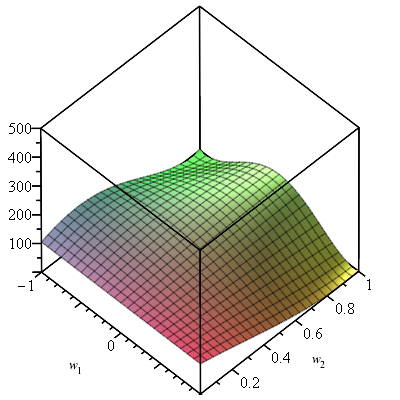
\includegraphics[width=0.33\linewidth]{graphics/nac-mul-nmu.png}
\caption{RMS loss curvature (without regularization) for a $\mathrm{NAC}_{+}$ layer followed by an $\mathrm{NMU}$ layer. Otherwise, the setup is identical to that in Figure \ref{fig:nac-mul-eps-issue}.}
\end{figure}

\subsection{Moments and initialization for addition}

Initialization is important for fast and consistent convergence. The desired properties are according to Glorot et al. \cite{glorot-initialization}:
\begin{equation}
\begin{aligned}
E[z_{h_\ell}] &= 0 & E\left[\frac{\partial \mathcal{L}}{\partial z_{h_{\ell-1}}}\right] &= 0 \\
Var[z_{h_\ell}] &= Var\left[z_{h_{\ell-1}}\right] &
Var\left[\frac{\partial \mathcal{L}}{\partial z_{h_{\ell-1}}}\right] &= Var\left[\frac{\partial \mathcal{L}}{\partial z_{h_{\ell}}}\right]
\end{aligned}
\end{equation}

The $\mathrm{NAC}_{+}$ layer is trivial, as this is just a linear layer. Thus the result from Glorot et al. ($Var[W_{h_{\ell-1},h_{\ell}}] = \frac{2}{H_{\ell-1} + H_{\ell}}$) can be used \cite{glorot-initialization}.

In the case of the $\mathrm{NAU}$, this condition is easy to satisfy. However, the original $\mathrm{NAC}_{+}$ unit is less trivial as $W_{h_{\ell-1},h_{\ell}}$ is not sampled directly. But assuming that $\hat{W}_{h_\ell, h_{\ell-1}} \sim \mathrm{Uniform}[-r, r]$ and $\hat{M}_{h_\ell, h_{\ell-1}} \sim \mathrm{Uniform}[-r, r]$ then the variance can be derived to be:
\begin{equation}
Var[W_{h_{\ell-1},h_{\ell}}] = \frac{1}{2r} \left(1 - \frac{\tanh(r)}{r}\right) \left(r - \tanh\left(\frac{r}{2}\right)\right)
\end{equation}
One can the solve for $r$, given the desired variance. 

\subsection{Moments and initialization for multiplication}

Using second order multivariate Taylor approximation and some assumptions of uncorrelated stochastic variables, the expectation and variance of the $\mathrm{NAC}_{\bullet}$ layer can be estimated to:
\begin{equation}
\begin{aligned}
f(c_1, c_2) &= \left(1 + c_1 \frac{1}{2} Var[W_{h_\ell, h_{\ell-1}}] \log(|E[z_{h_{\ell-1}}]| + \epsilon)^2\right)^{c_2\ H_{\ell-1}} \\
E[z_{h_\ell}] &\approx f\left(1, 1\right) \\
Var[z_{h_2}] &\approx f\left(4, 1\right) - f\left(1, 2\right) \\
E\left[\frac{\partial \mathcal{L}}{\partial z_{h_{\ell-1}}}\right] &= 0 \\
Var\left[\frac{\partial \mathcal{L}}{\partial z_{h_{\ell-1}}}\right] &\approx Var\left[\frac{\partial \mathcal{L}}{\partial z_{h_{\ell}}}\right] H_{\ell}\ f\left(4, 1\right)\ Var[W_{h_{\ell}, h_{\ell-1}}] \\
&\cdot \left(\frac{1}{\left(|E[z_{h_{\ell-1}}]| + \epsilon\right)^2} + \frac{3}{\left(|E[z_{h_{\ell-1}}]| + \epsilon\right)^4} Var[z_{h_{\ell-1}}]\right)
\end{aligned}
\end{equation}

This is problematic because $E[z_{h_\ell}] \ge 1$, and the variance explodes for $E[z_{h_{\ell-1}}] = 0$ which is normally a desired property.

For our proposed NMU, the expectation and variance can be derived using the same assumptions as before, although no Taylor approximation is required:
\begin{equation}
\begin{aligned}
E[z_{h_\ell}] &\approx \left(\frac{1}{2}\right)^{H_{\ell-1}} \\
E\left[\frac{\partial \mathcal{L}}{\partial z_{h_{\ell-1}}}\right] &\approx 0 \\
Var[z_{h_\ell}] &\approx \left(Var[W_{h_{\ell-1},h_\ell}] + \frac{1}{4}\right)^{H_{\ell-1}} \left(Var[z_{h_{\ell-1}}] + 1\right)^{H_{\ell-1}} - \left(\frac{1}{4}\right)^{H_{\ell-1}} \\
Var\left[\frac{\partial \mathcal{L}}{\partial z_{h_{\ell-1}}}\right] &\approx Var\left[\frac{\partial \mathcal{L}}{\partial z_{h_\ell}}\right] H_\ell \\
& \cdot \left( \left(Var[W_{h_{\ell-1},h_\ell}] + \frac{1}{4}\right)^{H_{\ell-1}} \left(Var[z_{h_{\ell-1}}] + 1\right)^{H_{\ell-1}-1} - \left(\frac{1}{4}\right)^{H_{\ell-1}}\right)
\end{aligned}
\end{equation}

These expectations are much more well behaved. It is properly unlikely to expect that the expectation can become zero, since the identity for multiplication is 1. However, for a large $H_{\ell-1}$ it will be near zero.

The variance is also more well-behaved, but does not provide a input-independent initialization strategy. We propose initializing with $Var[W_{h_{\ell-1},h_\ell}] = \frac{1}{4}$, as this is the solution to $Var[z_{h_\ell}] = Var[z_{h_{\ell-1}}]$ assuming $Var[z_{h_{\ell-1}}] = 1$ and a large $H_{\ell-1}$. However, feel free to compute more exact solutions.




\subsubsection*{Acknowledgments}

\blackout{Use unnumbered third level headings for the acknowledgments. All acknowledgments go at the end of the paper. Do not include acknowledgments in the anonymized submission, only in the final paper.}

\section*{References}
\bibliographystyle{plainnat}
\bibliography{bibliography}

\end{document}
